\exercisesheader{}

% 1

\eoce{\qt{Area under the curve, Part I\label{area_under_curve_1}} What percent of a 
standard normal distribution $N(\mu=0, \sigma=1)$ is found in each region? 
Be sure to draw a graph. \vspace{-3mm}
\begin{multicols}{4}
\begin{parts}
\item $Z < -1.35$
\item $Z > 1.48$
\item $-0.4 < Z < 1.5$
\item $|Z| > 2$
\end{parts}
\end{multicols}
}{}

% 2

\eoce{\qt{Area under the curve, Part II\label{area_under_curve_2}} What percent of 
a standard normal distribution $N(\mu=0, \sigma=1)$ is found in each region? 
Be sure to draw a graph. \vspace{-3mm}
\begin{multicols}{4}
\begin{parts}
\item $Z > -1.13$
\item $Z < 0.18$
\item $Z > 8$
\item $|Z| < 0.5$
\end{parts}
\end{multicols}
}{}

% 3

\eoce{\qt{GRE scores, Part I\label{GRE_intro}} Sophia who took the Graduate Record 
Examination (GRE) scored 160 on the Verbal Reasoning section and 157 on the 
Quantitative Reasoning section. The mean score for Verbal Reasoning section 
for all test takers was 151 with a standard deviation of 7, and the mean 
score for the Quantitative Reasoning was 153 with a standard deviation of 
7.67. Suppose that both distributions are nearly normal. 
\begin{parts}
\item Write down the short-hand for these two normal distributions.
\item What is  Sophia's Z-score on the Verbal Reasoning section? On the 
Quantitative Reasoning section? Draw a standard normal distribution curve and 
mark these two Z-scores.
\item What do these Z-scores tell you?
\item Relative to others, which section did she do better on?
\item Find her percentile scores for the two exams.
\item What percent of the test takers did better than her on the Verbal 
Reasoning section? On the Quantitative Reasoning section?
\item Explain why simply comparing raw scores from the two sections could lead 
to an incorrect conclusion as to which section a student did better on.
\item If the distributions of the scores on these exams are not nearly 
normal, would your answers to parts (b) - (f) change? Explain your reasoning.
\end{parts}
}{}

% 4

\eoce{\qt{Triathlon times, Part I\label{triathlon_times_intro}} In triathlons, it 
is common for racers to be placed into age and gender groups. Friends Leo and 
Mary both completed the Hermosa Beach Triathlon, where Leo competed in the 
\textit{Men, Ages 30 - 34} group while Mary competed in the \textit{Women, 
Ages 25 - 29} group. Leo completed the race in 1:22:28 (4948 seconds), while 
Mary completed the race in 1:31:53 (5513 seconds). Obviously Leo finished 
faster, but they are curious about how they did within their respective 
groups. Can you help them? Here is some information on the performance of 
their groups:
\begin{itemize}
\setlength{\itemsep}{0mm}
\item The finishing times of the \textit{Men, Ages 30 - 34} group has a mean 
of 4313 seconds with a standard deviation of 583 seconds.
\item The finishing times of the \textit{Women, Ages 25 - 29} group has a 
mean of 5261 seconds with a standard deviation of 807 seconds.
\item The distributions of finishing times for both groups are approximately 
Normal.
\end{itemize}
Remember: a better performance corresponds to a faster finish.
\begin{parts}
\item Write down the short-hand for these two normal distributions.
\item What are the Z-scores for Leo's and Mary's finishing times? What do 
these Z-scores tell you?
\item Did Leo or Mary rank better in their respective groups? Explain your 
reasoning.
\item What percent of the triathletes did Leo finish faster than in his group?
\item What percent of the triathletes did Mary finish faster than in her 
group?
\item If the distributions of finishing times are not nearly normal, would 
your answers to parts (b)~-~(e) change? Explain your reasoning.
\end{parts}
}{}

% 5

\eoce{\qt{GRE scores, Part II\label{GRE_cutoffs}} In Exercise~\ref{GRE_intro} we 
saw two distributions for GRE scores: $N(\mu=151, \sigma=7)$ for the verbal 
part of the exam and $N(\mu=153, \sigma=7.67)$ for the quantitative part. Use 
this information to compute each of the following:
\begin{parts}
\item The score of a student who scored in the $80^{th}$ percentile on the 
Quantitative Reasoning section.
\item The score of a student who scored worse than 70\% of the test takers in 
the Verbal Reasoning section.
\end{parts}
}{}

% 6

\eoce{\qt{Triathlon times, Part II\label{triathlon_times_cutoffs}} In 
Exercise~\ref{triathlon_times_intro} we saw two distributions for triathlon 
times: $N(\mu=4313, \sigma=583)$ for \emph{Men, Ages 30 - 34} and 
$N(\mu=5261, \sigma=807)$ for the \emph{Women, Ages 25 - 29} group. Times are 
listed in seconds. Use this information to compute each of the following:
\begin{parts}
\item The cutoff time for the fastest 5\% of athletes in the men's group, i.e. those 
who took the shortest 5\% of time to finish. 
\item The cutoff time for the slowest 10\% of athletes in the women's group. 
\end{parts}
}{}

% 7

\eoce{\qt{LA weather, Part I\label{la_weather_intro}} \videohref{ahss_eoce_sol-la_weather_intro}\ \ The average daily high 
temperature in June in LA is 77\degree F with a standard deviation of 
5\degree F. Suppose that the temperatures in June closely follow a normal 
distribution. 
\begin{parts}
\item What is the probability of observing an 83\degree F temperature or 
higher in LA during a randomly chosen day in June?
\item How cool are the coldest 10\% of the days (days with lowest average 
high temperature) during June in LA?
\end{parts}
}{}

% 8

\eoce{\qt{CAPM\label{CAPM}} The Capital Asset Pricing Model (CAPM) is a financial 
model that assumes returns on a portfolio are normally distributed. Suppose a 
portfolio has an average annual return of 14.7\% (i.e. an average gain of 
14.7\%) with a standard deviation of 33\%. A return of 0\% means the value of 
the portfolio doesn't change, a negative return means that the portfolio 
loses money, and a positive return means that the portfolio gains money.
\begin{parts}
\item What percent of years does this portfolio lose money, i.e. have a 
return less than 0\%?
\item What is the cutoff for the highest 15\% of annual returns with this 
portfolio?
\end{parts}
}{}

% 9

\eoce{\qt{LA weather, Part II\label{la_weather_unit_change}} 
Exercise~\ref{la_weather_intro} states that average daily high temperature in 
June in LA is 77\degree F with a standard deviation of 5\degree F, and it can 
be assumed that they to follow a normal distribution. We use the following 
equation to convert \degree F (Fahrenheit) to \degree C (Celsius):
\[ C = (F - 32) \times \frac{5}{9}. \]
\begin{parts}
\item Write the probability model for the distribution of temperature in 
\degree C in June in LA.
\item What is the probability of observing a 28\degree C (which roughly 
corresponds to 83\degree F) temperature or higher in June in LA? Calculate 
using the \degree C model from part (a).
\item Did you get the same answer or different answers in part (b) of this 
question and part (a) of Exercise~\ref{la_weather_intro}? Are you surprised? Explain.
\item Estimate the IQR of the temperatures (in \degree C) in June in LA.
\end{parts}
}{}

% 10

\eoce{\qt{Find the SD\label{find_sd}} Cholesterol levels for women aged 20 to 34 follow an approximately 
normal distribution with mean 185 milligrams per deciliter (mg/dl). Women 
with cholesterol levels above 220 mg/dl are considered to have high 
cholesterol and about 18.5\% of women fall into this category.  Find the standard deviation of this distribution.
}{}


% 11

\eoce{\qt{Scores on stats final, Part I} \label{statsScores} Below are final exam scores of 20 Introductory Statistics students. 
\[ \stackrel{1}{57}, \stackrel{2}{66}, \stackrel{3}{69}, \stackrel{4}{71}, \stackrel{5}{72}, \stackrel{6}{73}, \stackrel{7}{74}, \stackrel{8}{77}, \stackrel{9}{78}, \stackrel{10}{78}, \stackrel{11}{79}, \stackrel{12}{79}, \stackrel{13}{81}, \stackrel{14}{81}, \stackrel{15}{82}, \stackrel{16}{83}, \stackrel{17}{83}, \stackrel{18}{88}, \stackrel{19}{89}, \stackrel{20}{94} \]
The mean score is 77.7 points. with a standard deviation of 8.44 points. Use this information to determine if the scores approximately follow the 68-95-99.7\% Rule.
}{}

% 12

\eoce{\qt{Heights of female college students, Part I} \label{collegeFemHeights} Below are heights of 25 female college students.
\[ \stackrel{1}{54}, \stackrel{2}{55}, \stackrel{3}{56}, \stackrel{4}{56}, \stackrel{5}{57}, \stackrel{6}{58}, \stackrel{7}{58}, \stackrel{8}{59}, \stackrel{9}{60}, \stackrel{10}{60}, \stackrel{11}{60}, \stackrel{12}{61}, \stackrel{13}{61}, \stackrel{14}{62}, \stackrel{15}{62}, \stackrel{16}{63}, \stackrel{17}{63}, \stackrel{18}{63}, \stackrel{19}{64}, \stackrel{20}{65}, \stackrel{21}{65}, \stackrel{22}{67}, \stackrel{23}{67}, \stackrel{24}{69}, \stackrel{25}{73} \]
The mean height is 61.52 inches with a standard deviation of 4.58 inches. Use this information to determine if the heights approximately follow the 68-95-99.7\% Rule.
}{}

% 13

\eoce{\qt{Scores on stats final, Part II} Exercise~\ref{statsScores} lists the final exam scores of 20 Introductory Statistics students. Do these data appear to follow a normal distribution? Explain your reasoning using the graphs provided below.
\begin{center}
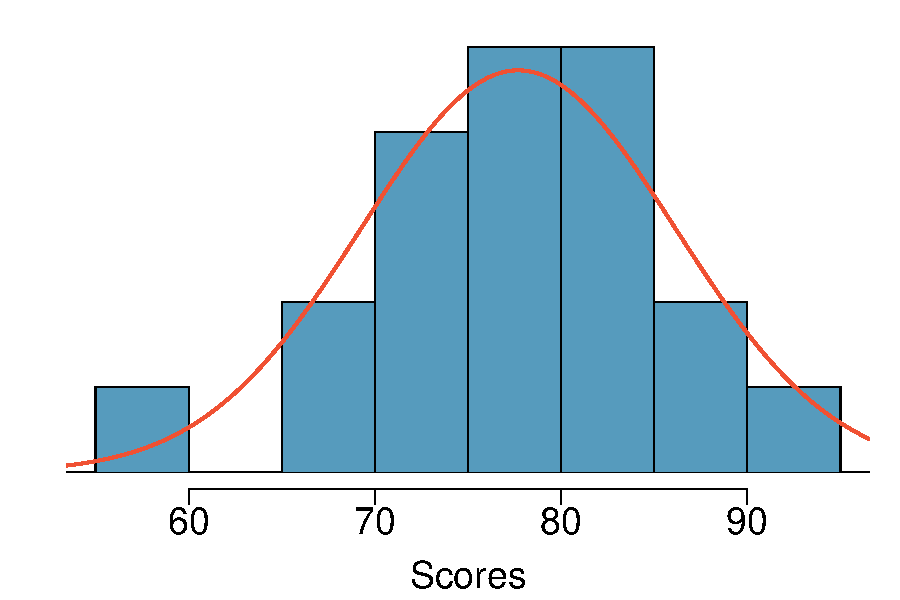
\includegraphics[width=0.46\textwidth]{ch_distributions/figures/eoce/scores/scores_hist}\ \ \ \ 
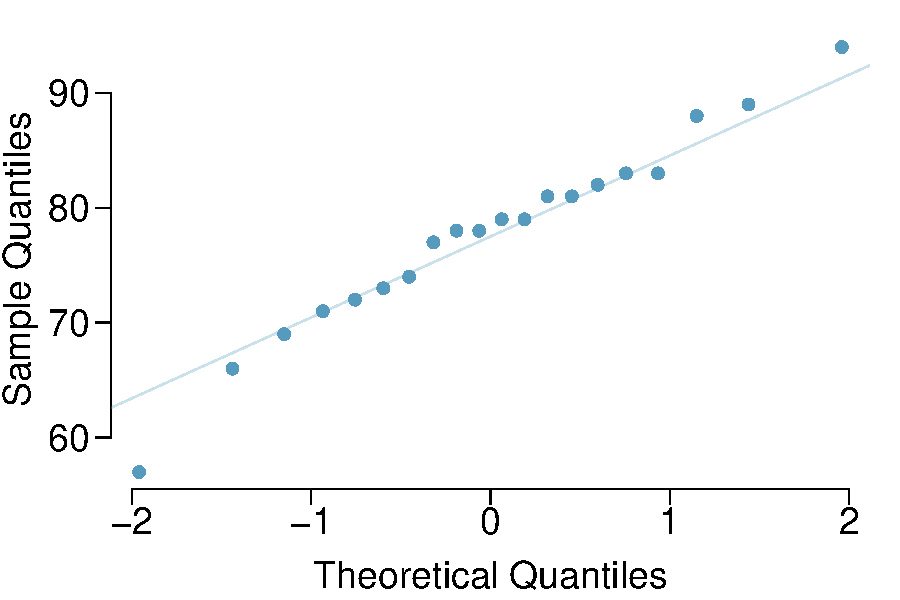
\includegraphics[width= 0.46\textwidth]{ch_distributions/figures/eoce/scores/scores_qq}
\end{center}
}{}

% 14

\eoce{\qt{Heights of female college students, Part II} Exercise~\ref{collegeFemHeights} lists the heights of 25 female college students. Do these data appear to follow a normal distribution? Explain your reasoning using the graphs provided below.
\begin{center}
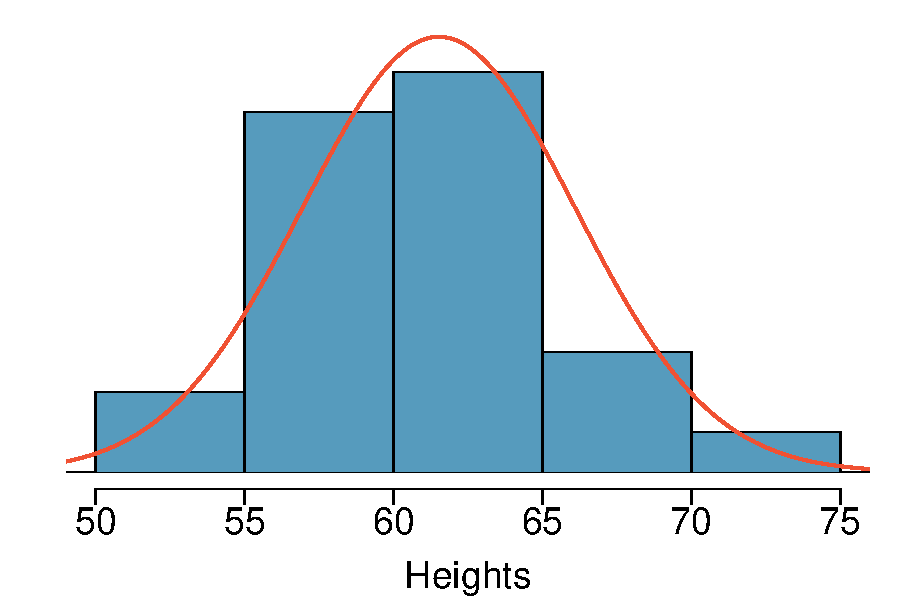
\includegraphics[width= 0.46\textwidth]{ch_distributions/figures/eoce/heightsFcoll/heightsFcoll_hist}\ \ \ \ 
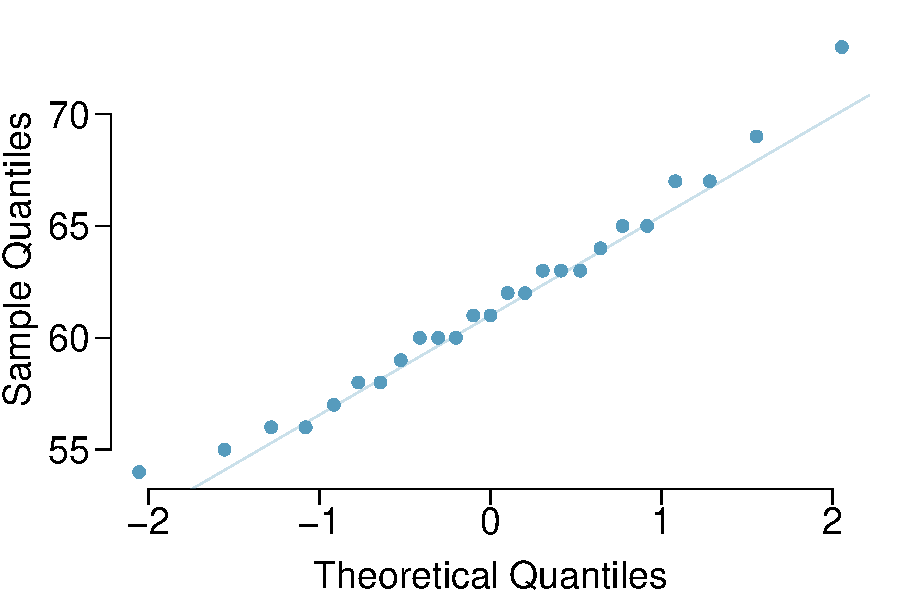
\includegraphics[width= 0.46\textwidth]{ch_distributions/figures/eoce/heightsFcoll/heightsFcoll_qq}
\end{center}
}{}

\textA{\pagebreak}

% 15

\eoce{\qt{Lemonade at The Cafe} Drink pitchers at The Cafe are intended to hold about 64 ounces of lemonade and glasses hold about 12 ounces. However, when the pitchers are filled by a server, they do not always fill it with exactly 64 ounces. There is some variability. Similarly, when they pour out some of the lemonade, they do not pour exactly 12 ounces. The amount of lemonade in a pitcher is normally distributed with mean 64 ounces and standard deviation 1.732 ounces. The amount of lemonade in a glass is normally distributed with mean 12 ounces and standard deviation 1 ounce. 
\begin{parts}
\item How much lemonade would you expect to be left in a pitcher after pouring one glass of lemonade? 
\item What is the standard deviation of the amount left in a pitcher after pouring one glass of lemonade? 
\item What is the probability that more than 50 ounces of lemonade is left in a pitcher after pouring one glass of lemonade?
\end{parts}
}{}

% 16

\eoce{\qt{Spray paint, Part I} \label{sprayPaint} Suppose the area that can be painted using a single can of spray paint is slightly variable and follows a nearly normal distribution with a mean of 25 square feet and a standard deviation of 3 square feet. Suppose also that you buy three cans of spray paint.
\begin{parts}
\item How much area would you expect to cover with these three cans of spray paint?
\item What is the standard deviation of the area you expect to cover with these three cans of spray paint?
\item The area you wanted to cover is 80 square feet. What is the probability that you will be able to cover this entire area with these three cans of spray paint?
\end{parts}
}{}

% 17

\eoce{\qt{GRE scores, Part III} \videohref{ahss_eoce_sol-gre_scores_part_III}\ \ In Exercise~\ref{GRE} we saw two distributions for GRE scores: $N(\mu=151, \sigma=7)$ for the verbal part of the exam and $N(\mu=153, \sigma=7.67)$ for the quantitative part. Suppose performance on these two sections is independent. Use this information to compute each of the following:
\begin{parts}
\item The probability of a combined (verbal + quantitative) score above 320. 
\item The score of a student who scored better than 90\% of the test takers overall.
\end{parts}
}{}

% 18
\eoce{\qt{Betting on dinner, Part I} \label{dinnerBet} Suppose a restaurant is running a promotion where prices of menu items are determined randomly following some underlying distribution. This means that if you're lucky you can get a basket of fries for \$3, or if you're not so lucky you might end up having to pay \$10 for the same menu item. The price of basket of fries is drawn from a normal distribution with mean 6 and standard deviation of 2. The price of a fountain drink is drawn from a normal distribution with mean 3 and standard deviation of 1. What is the probability that you pay more than \$10 for a dinner consisting of a basket of fries and a fountain drink?}
{}

